\section{TP: Automatisons des tâches avec Makefile, Illustration pour  \LaTeX }

On a vu et on verra des commandes à exécuter dans un terminal pour
résoudre un certain nombre de problèmes (vérifier l'orthographe d'un
texte, travailler des images, regrouper des images pour créer une
vidéo, lister/modifier un ensemble de fichiers, compiler un document
\LaTeX, compiler un programme, ...). Il peut devenir difficile de se souvenir de la syntaxe
d'une commande et la syntaxe peut même devenir compliquée quand on
souhaite enchaîner des commandes. GNU Make est un des outils qui
permet d'automatiser l'exécution de tâches. L'outil \make est installé
avec le paquet \emph{make} et en général installé par défaut avec la
distribution. L'utilisation de \make passe par la
définition de fichiers Makefile qui sont traités par la commande \make. Ces fichiers peuvent s'appeler
\emph{GNUmakefile}, \emph{makefile}, ou \emph{Makefile}. Ils
contiennent un ensemble de règles avec une forme canonique:
\begin{verbatim}
cible: dépendances
       commandes
\end{verbatim}
Une règle doit être comprise comme définissant une recette de cuisine (les
commandes) permettant de construire une cible si les dépendances ont
changées. Les dépendances sont optionnelles, on en verra un exemple un
peu plus loin. \textbf{Attention} chaque ligne de \underline{commande} doit être
précédée par une tabulation. On considère un exemple
assez standard pour illustrer quelques concepts de Make, celui de
compiler un document \LaTeX. Si on veut compiler un document \LaTeX \emph{document.tex} "à la main", il faut appeler plusieurs fois \pdflatex. Si vous n'avez aucune référence bibliographique (i.e. vous n'appelez jamais ``\textbackslash{}cite") dans votre document mais des références croisées (i.e. vous appelez au moins une fois ``\textbackslash{}ref", par exemple pour faire référence à une image ou une section), il faut lancer deux fois la commande \pdflatex: le premier appel produit un fichier de référence (document.aux), le deuxième remplace chaque référence par son label. Si vous avez des références bibliographiques, il faut lancer \pdflatex, \bibtex, et \pdflatex deux fois. Comme dans le premier cas, le premier appel à \pdflatex produit une liste des références (bibliographiques et croisées) dans le fichier document.aux. L'appel à \bibtex prend en entrée le fichier document.aux, met en forme la bibliographie et produit le fichier document.bbl. Il faut maintenant intégrer cette bibliographie à votre document; c'est ce que fait l'appel suivant à \pdflatex. Enfin, un dernier appel à \pdflatex est nécessaire pour assigner, dans le document, le texte associé à une citation (son numéro par exemple). Pour résumer, pour compiler un document \LaTeX à la main, il faut exécuter, depuis un terminal, les commandes suivantes~:
\begin{center}
\bash{pdflatex document.tex ; bibtex document
  ; pdflatex document.tex; pdflatex document.tex}
\end{center}
Vous m'accorderez que c'est un peu fastidieux. Avec \make, on peut se simplifier la vie, c'est ce que nous allons voir.\\

\subsection{Première compilation d'un fichier \LaTeX avec un Makefile}

\textbf{Commencez} par récupérer un template \LaTeX qui vous plait \underline{de la section Articles} depuis le site \url{http://www.latextemplates.com/}. Je vous demande de prendre un exemple de la section Articles pour être sûr qu'il contienne des références bibliographiques. Faites l'extraction de l'archive quelque part sur votre home. Appelons par la suite ce répertoire \emph{Document}. Renommez le fichier .tex de l'archive en \emph{document.tex}. Définissez vous un fichier intitulé Makefile (sans extension, c'est pas grave!), dans lequel vous metterez le texte ci-dessous~:\\
\cprotect\encadreUtilisation{ Fichier  \textbf{Makefile}
\begin{verbatim}
document.pdf: document.tex
              pdflatex document.tex 
              bibtex document
              pdflatex document.tex 
              pdflatex document.tex
\end{verbatim}
}
Que dit cette règle ? Elle dit que la cible document.pdf dépends de la cible document.tex. Ainsi, si vous souhaitez produire la cible document.pdf mais que document.tex n'a pas changé depuis la dernière production de document.pdf, \make vous dira simplement qu'il n'y a rien à faire, i.e. on ne perds pas de temps à recompiler le document puisque son contenu n'a pas changé! Au contraire, si document.tex a changé, \make exécutera la recette de cuisine pour générer la cible document.pdf. Pour compiler votre document, il vous suffit de taper, dans le terminal \bash{make document.pdf},  et de laisser \LaTeX mouliner. Si tout s'est bien passé, vous devriez voir un fichier \emph{document.pdf} que vous pouvez ouvrir grâce à la commande \bash{evince document.pdf}\footnote{sur certaines distributions, il existe d'autres viewers PDF, comme \okular, sous Ubuntu. L'un des avantages des viewers comme \okular ou \evince, et comparé à \acroread, c'est qu'il se met automatiquement à jour si le document PDF est regénéré.}.\\

Pour se simplifier encore un peu la vie, on peut ajouter une autre règle~:\\
\cprotect\encadreUtilisation{ Fichier  \textbf{Makefile}\\
(...)
\begin{verbatim}
pdf: document.pdf
\end{verbatim}
}
Ici, c'est une règle sans recette de cuisine, juste une dépendance. Mais pour le coup, il vous suffit de taper \bash{make pdf} pour produire le document PDF.

\subsection{Une règle pour faire le ménage}

\textbf{Listez} les éléments du répertoire et vous devriez constater que nos appels à \pdflatex et \bibtex ont produits plusieurs fichiers temporaires (des fichiers .aux, .bbl, .out, .log, ...). Il y a également des fichiers temporaires produits par \emacs que vous avez utilisé pour éditer votre fichier latex et votre Makefile: ce sont les fichiers qui se terminent avec un tilde, e.g.  "document.tex\textasciitilde".\\

Pour supprimer les fichiers temporaires, il suffit de lancer la commande~: \bash{rm document.aux document.bbl document.out document.log document.tex\textasciitilde}. \underline{\textbf{ATTENTION!!}} N'oubliez pas le tilde à la fin de document.tex sinon, ben vous supprimez votre document.... \textbf{Définissez} une règle dont la cible est \emph{clean}, qui n'a pas de dépendance, et dont la recette de cuisine supprime les fichiers temporaires. \textbf{Testez la}, ça marche ?\\

\subsection{Et voila}

Finalement, le Makefile précédent est tout ce dont nous avons besoin pour produire du PDF à partir d'un fichier \LaTeX. En résumé, si vous voulez écrire en \LaTeX, il vous faut~:
\begin{itemize}
\item un bon éditeur de texte avec correction orthographique, e.g. \emacs (qui peut d'ailleurs également éditer des fichiers bitex)
\item un viewer de document PDF, e.g. \evince ou \okular
\item un Makefile pour automatiser la compilation
\end{itemize}

En passant, vous pouvez aussi réaliser des supports de présentation avec \LaTeX grâce au paquet Beamer ou dérivés. Allez voir sur le site \url{www.latextemplates.com}, dans la section Presentations.


\subsection{Allons un peu plus loin}

La règle de compilation d'un document \LaTeX est assez générique, elle n'est pas spécifique au document document.tex mais pourrait s'appliquer à n'importe quel document latex avec l'extension .tex. Avec \make, on peut définir des règles génériques et je vous propose de chercher à l'écrire en vous renvoyant à la section \ref{sec:makefile} dans laquelle cette question est abordée dans le contexte de la compilation de programme C++. \\

Enfin, sur un autre sujet, sachez que si vous souhaitez créer des illustrations dans lesquelles faire apparaître des formules mathématiques \LaTeX, vous pouvez le faire grâce à un logiciel de dessin vectoriel, certes sobre, mais très pratique: \xfig. D'ailleurs, sachez également que les dessins \xfig sont générables "à la main", c'est à dire qu'un programme peut écrire une série de commandes de tracé directement en format ASCII et vous pourrez alors importer votre figure depuis \xfig ou l'exporter vers d'autres formats (de préférence vectoriel: svg, eps, ..).

%% \subsection{En passant, et si vous vouliez faire des figures avec des notations mathématiques ?}

%% Dans la série des programmes qui peuvent paraître austaires mais qui rendent bien service, je vous propose de regarder \xfig.

%% \begin{figure}[htbp]
%% 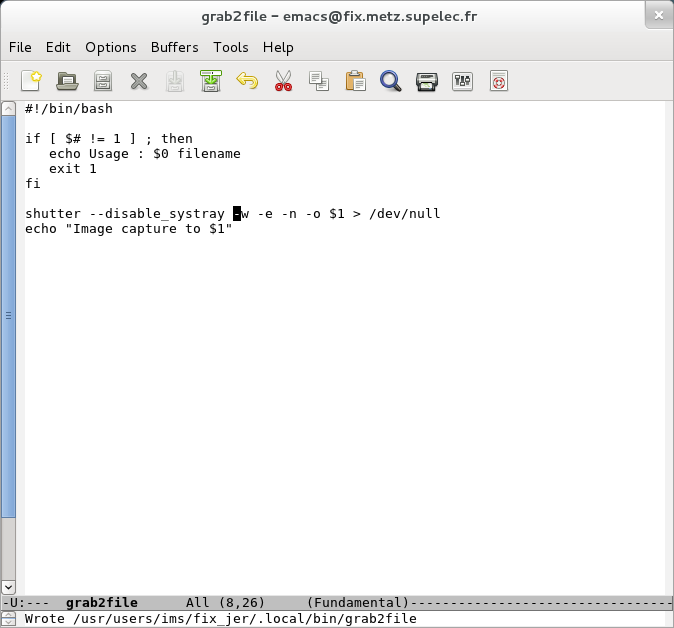
\includegraphics[width=0.5\columnwidth]{test.pdf}
%% \end{figure}
